% This version of CVPR template is provided by Ming-Ming Cheng.
% Please leave an issue if you found a bug:
% https://github.com/MCG-NKU/CVPR_Template.

\documentclass[review]{cvpr}
%\documentclass[final]{cvpr}

\usepackage{times}
\usepackage{epsfig}
\usepackage{graphicx}
\usepackage{amsmath}
\usepackage{amssymb}

% Include other packages here, before hyperref.

% If you comment hyperref and then uncomment it, you should delete
% egpaper.aux before re-running latex.  (Or just hit 'q' on the first latex
% run, let it finish, and you should be clear).
\usepackage[pagebackref=true,breaklinks=true,colorlinks,bookmarks=false]{hyperref}

\usepackage[ruled,vlined]{algorithm2e}

% Include other packages here, before hyperref.

% If you comment hyperref and then uncomment it, you should delete
% egpaper.aux before re-running latex.  (Or just hit 'q' on the first latex
% run, let it finish, and you should be clear).
\usepackage[breaklinks=true,bookmarks=false]{hyperref}


\def\cvprPaperID{****} % *** Enter the CVPR Paper ID here
\def\confYear{CVPR 2021}
%\setcounter{page}{4321} % For final version only


\begin{document}


%%%%%%%%% TITLE
\title{SmallDepthMask: Large DataSet Generation for Monocular Depth Estimation and Foreground Segmentation from few Internet Images
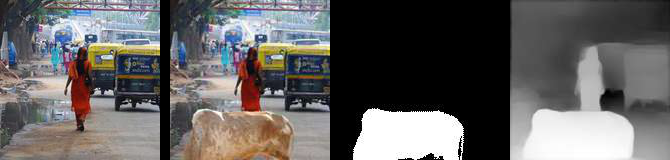
\includegraphics[width=1\textwidth]{samplerecord.png}
}

\author{Sridevi Bonthu\\
Vishnu Institute of Technology\\
Bhimavaram, AP, India 534202\\
{\tt\small sridevi.b@vishnu.edu.in}
% For a paper whose authors are all at the same institution,
% omit the following lines up until the closing ``}''.
% Additional authors and addresses can be added with ``\and'',
% just like the second author.
% To save space, use either the email address or home page, not both
\and
Abhinav Dayal\\
Vishnu Institute of Technology\\
Bhimavaram, AP, India 534202\\
{\tt\small abhinav.dayal@vishnu.edu.in}
}

\maketitle
%\thispagestyle{empty}

%%%%%%%%% ABSTRACT
\begin{abstract}
  Segmentation of the desired object along with depth estimation is useful in various applications like robotics and autonomous navigation. 
  Any deep learning workflow to segment the desired foreground object in a scene require significant training data.
  The data generation process usually involve expensive hardware like RGB-D sensors, Laser Scanners or significant manual involvement. 
  This paper presents a novel way to utilize only a small number of readily available png images with transparency for the foreground object, 
  and representative background images from the internet and combine them to generate a huge dataset for deep learning
  utilizing current state of the art monocular depth estimation and segmentation techniques. 
  Few example applications show the efficacy of the training data on detecting 
  cattle on road for autonomous driving application, etc. The baseline models exhibit strong generalization to real scenarios.
\end{abstract}

%Keywords : Large Dataset, Depth image, Segmentation Mask, Depth prediction, Custom Dataset, Baseline model.
 

%%%%%%%%% BODY TEXT
\section{Introduction}
%Expand the abstract with appropriate references. We need references for:
%1. Monocular Depth
%2. Image segmentation
%3. Deep learning requiring large datasets
%4. Generating data sets is cumbersome
%5. Ours is novel work that uses few images to generate huge dataset that generalizes well
%Above From Abhinav
%Depth information and Image segmentation are highly correlated and both are equally 
%important in challenging applications which involve identification of objects as well as their distance 
%from the camera and 3D reconstruction..
% need for depth estimation and segmentation (some application references). 
% How deep learning require large datasets to learn - challenges with that
% What kind of datasets are generated for this application
% Generating data sets is cumbersome, what are some of the current ways. Many doing depth or only segmentation, 
% however depth along with mask for desired foreground objects is forst of kind
Depth estimation and semantic segmentation are often used together in many vision tasks~\cite{lin2018joint} like 
autonomous navitation of agents, augmented reality, self driving cars and other robotics applications. In all these application,
identification of desired objects precisely in the scene and its depth estimate from the camera are crucial for safe and effective
navigation. Modern RGB-D sensors like OAK-D are capable of simultaneously running advanced neural networks while providing depth 
from two stereo cameras and color information from a single 4K camera in the center. Deep learning based techniues using convolution
neural nets have effective solution in both depth estimation and semantic segmentation. In general for high accuracy outcomes, a
deep learning network is dependent on large training dataset availability. To gather such data itself incur high cost and time.
For specific applications requiring several forground objects against variety of backgrounds become even more challenging in terms
of simulating those scenarioes. Synthetic datasets using Virtual Reality have been proposed to that end.

Recent research indicates effective use of readily available images on the internet to curate training data.  
This paper introduces SmallDepthMask, 
a way to curate custom dataset containing millions of images by multiplexing desired foreground objects over representative background 
scenes, while also generating corresponding depth and foreground mask images. This significantly reduces the cost and time overheads.
The authors also experiment by creating baseline models for several application contexts and show that the generated data
successfully generalizes to detect relevant objcts in real scenes. Multiplexing, combined with random cropping, scaling 
and translation, make the datageneration fast and effective. With only 100 pair of background and foregroung images, the authors
generate 4 million image triplets and effectively leverage existing SOTA models for depth estimation and semantic segmentation.

The main contributions of this paper are the following:
\begin{enumerate}
\item A novel effort to mix and match foreground and background images reducing the need for complex scene generation for data curation.
\item Curate large dataset to effectively train models for custom applications of detecting depth and mask for specific foreground objects over any target background, from a limited input of ready available internet images.
\item Combine image, depthmap and forground mask in a single dataset using current SOTA models for depth estimation and semantic segmentation.
\item To release curated dataset and the trained models making them publicly available. Researchers can use this single dataset to do segmentation, 
train models to predict depth, or to predict both depth and mask.
\end{enumerate}
  

Figure \ref{fig:sampledatarecord} represents an example from the generated dataset to help detect cattle on road,
 which is very common on Indian roads, leading to several accidents involving loss of life and property. 
 The generated datasets and the trained models are publicly available.


%The datasets which involve depth cannot be 
%created using crowd source annotation, instead they rely on 3D range sensors. SmallDepthMask is experimentally created 
%with the help of existing depth predictors and foreground creators.



%A para on the organization of the paper.......................................


\section {Related Work}

A depth image is an image channel in which each pixel relates to a distance between the image plane and the
corresponding object in the RGB image.
Monocular depth gives information about depth and distance and the Monocular Depth Estimation is the task of estimating scene depth 
using a single image\cite{abuolaim2020defocus}. 
Image Segmentation is the process of partitioning an image into multiple segements and it can be used for locating objects, 
boundaries~\cite{amza2012review}. RGBD image is a combination of a RGB image and its corresponding depth image\cite{zhang2018deep}.
 
Depth information is integral to many problems in
robotics including mapping, localization and obstacle avoidance for terrestrial and aerial vehicles, autonomous navigation, 
and in computer vision, including augmented and virtual reality\cite{marchand2015pose}. RGBD datasets usually collected 
using depth sensors, monocular cameras and LiDAR scanners are expensive and data collection is a time consuming job. 
The wellknown datasets for monocular 3D object detection are Context-Aware MixEd ReAlity (CAMERA), Objectron, 
Kitty3D, Cityscape3D, Synthia, etc.~\cite{} and these datasets have 
 limitations like indoor only images, small number of training examples and sparse sampling. 
 
 To address the issues usage of expensive devices and small number of training examples, this paper proposes a 
 technique to come up with a custom dataset by using existing accurate depth predictor models, like High Quality Monocular Depth Estimation 
 via Transfer Learning(nyu.h5)~\cite{alhashim2018high}. 

A variety of RGBD datasets in which images are paired with corresponding depth maps(D) have been proposed through the years.
Some of the frequenlty used RGBD datasets are the Kitti dataset~\cite{geiger2013vision}, the Synthia dataset~\cite{ros2016synthia}, 
Make3D dataset~\cite{saxena2008make3d}, NYU dataset~\cite{silberman2012indoor}

The dataset Kiiti~\cite{geiger2013vision} is the well known RGB-D dataset collected using a vehicle equipped with a sparse 
Velodyne VLP-64 LiDAR scanner and RGB cameras, and features street scenes in and around the German city of Karlsruhe. 
The Primary application of this dataset involves perception tasks in the context of self-driving. 
Synthia~\cite{ros2016synthia} is a street scene dataset with depth maps of synthetic data, 
requiring domain adaptiation to apply to 
real world settings. Cityscapes~\cite{cordts2016cityscapes} provides a dataset of street scenes, 
albeit with more diversity than KITTI. 
Sintel~\cite{mayer2016large} is another synthetic dataset which mainly comprises of outdoors sences.

Megadepth~\cite{li2018megadepth} is a large-scale dataset of outdoor images collected from internet, with depth maps reconstructed 
using structure-from-motion techniques, but this dataset lacks in ground truth depth and scale. The RedWeb~\cite{xian2018monocular}
dataset provide depth maps generated from stereo images which are freely available in large-scale data platforms such as Flicker. 
The datasets MegaDepth and RedWeb can be easily computed with the existing MVS methods.

Make3D~\cite{saxena2008make3d} provides RGB and depth information for outdoor scenes. 
The NYUv2 dataset~\cite{silberman2012indoor} is widely used for monocular depth estimation in indoor environments. 
The data was collected with a Kinect RGBD camera, which provides sparse and noisy depth returns. 
These returns are generally in-painted and smoothed before they are used for monocular depth estimation tasks. 
As a result, while the dataset includes sufficient samples to train modern machine learning pipelines,
the “ground-truth” depth does not necessarily correspond to true scene depth.

Most of the existing datasets consists of indoor images, or outdoor images of city streets. For every specific application, like
detecting animals roaming on roads for self driving or assisted driving cars, or people inside a room for autonomus room cleaners etc.
researchers need to curate specific dataset to train relevant deep learning models. The present work makes the task of 
curating dtaset extremely simple and cost effective.

\section{Method}
The curated dataset must have following objectives:
\begin{enumerate}
\item dataset which dedicatedly includes foreground object. 
\item dataset should drive deep learning models and generalize. 
\item dataset should provide accurate dense depth maps.
\item dataset should provide foreground mask
\item dataset can be stored offline or generated online during training phase dynamically
\end{enumerate}

\subsection{Data Acquisition}
The first step to curate data is to determine a target application scenario and thus determine the foreground object(s) and the
representative background context. At the same time the dataset must have sufficient variability to include majority of
the types and views that the trained deep network may see when deployed.

We propose to download or take RGB image of $n$ foreground object(s) and $m$ background images (we used $n=m=100$)
balancing the types and views. For example, for cattle on roads dataset, we shose several cow, bull and calf types, individual
 or in group, sitting, standing or walking, and from various angles. Similarly for background, we chose backgrounds of streets, 
 storefronts, main roads, highways, markets, railway tracks, landscapes, garbage piles etc.
PNG images with transparency are readily available on the internet for almost any desired foreground object.
Such images will easily allow to generate foreground mask from non-transparent pixels. 
If not, tools like GIMP~\cite{howat2014greenland}, combined with deep learning forground extractors\footnote{https://www.remove.bg/}
that uses a combination of Image based techniques .
and DNN to separate foreground from background) can help generate the required PNG foreground images.

\begin{figure*}
  \begin{center}
  \begin{tabular}{@{}c@{}}
    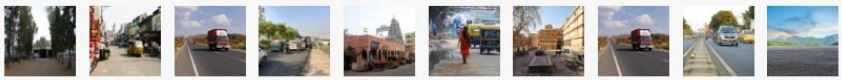
\includegraphics[width=1.0\linewidth]{bgimages.jpg}
  \end{tabular}
  \begin{tabular}{@{}c@{}}
      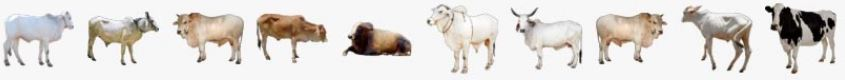
\includegraphics[width=1.0\linewidth]{fgimages.jpg}
  \end{tabular}
  \end{center}
  \caption{Scene and foreground object images}
  \label{fig:sceneandfg}
\end{figure*}

Fig.~\ref{fig:sceneandfg} shows few of the sample scene and foreground images used for the creation of this dataset. 

\subsection{Multiplexing and Depth Generation}

This step is to place each foreground object on to several background images generating a fg-bg image and the corresponding mask
corresponding to the foreground placement and scale. Depth is computed from the fg-bg image via the model proposed by 
Ibraheem Alhashim et al. in their paper titled "High Quality Monocular Depth Estimation via Transfer Learning"
~\cite{alhashim2018high}\footnote{source code for depth estimation model: https://github.com/ialhashim/DenseDepth/blob/master/DenseDepth.ipynb}. 
This model takes $448\times448$ size images as input, hence we resize all backfround images to this size while maintaining their aspect ratio.

The data generation process is completely online and produces one batch of images for training a deep model.
By repeating one forground object $k$ times for each background image and repeating another $k$ times with horizontally
flipped version of the same foreground, one can generate $2kmn$ fg-bg images. 
For $k=20$ and $n=m=100$ this becomes $400,000$ fg-bg images. Algorithm \ref{algo:datagen} describes the data generation process

\IncMargin{1em}
\begin{algorithm*}
  \label{algo:datagen}
  \SetKwData{Left}{left}\SetKwData{This}{this}\SetKwData{Up}{up}
  \SetKwFunction{Union}{Union}\SetKwFunction{FindCompress}{FindCompress}
  \SetKwInOut{Input}{input}\SetKwInOut{Output}{output}
  \Input{$m$ Background Image paths, $2n$ Foreground Image paths, multiplexing factor $k$, batch size $b$ \emph{must be multiple of $k$}}
  \Output{Yield $2kmn$ fg-bg, mask and depth images in batches of size $b$}
  \BlankLine
  \emph{for offline use it creates 3 folders with fg\_bg, mask and depth each having $2kmn$ images}\;

  \For{$bg\leftarrow 1$ \KwTo $m$}{
    \For{$fg\leftarrow 1$ \KwTo $2n$}{
      \For{$i\leftarrow 1$ \KwTo $k$}{
        $croppedbg\leftarrow$ take maximal random crop of $448\times448$ from $bg$ without affecting the aspect ratio\;
        randomly pick a center point $(x, y)$ in range $[0,447]$\;
     	  randomly pick a scale in range $[0.3, 0.6]$ (ratio of area $fg$ covers $bg$)\;
     	  create $fg-bg$ image by resizing the $fg$ to scale and place it on top of $croppedbg$ centered at $x, y$ calculated\;
        calculate binary mask from current placement of $fg$ by thresholding transparency channel.
        save $fg-bg$ image and mask
        add $fg-bg$ image to a batch\;
    }
    \If{$b$ new fg-bg images generated}{
      run depth model on batch and save corresponding depth images. Rescale saved images to $224\times224$
    }
    }}
\caption{Generate Dataset(\textit{[bgimages]}, \textit{[fgimages]}, $k$, $b$)}
\end{algorithm*}


%The Related work says that the depth measurement took place with variety of devices like kinects, structure light cameras, and LiDAR etc. 
%This work mainly focusing on the generation of huge dataset with limited availability of scene images and foreground images. 



% \subsection{Data Curation and Processing}
% % this may not be required

% Fig.~\ref{fig:finaldataset} shows the three outcomes of the above algorithm for a set of images.

% \subsubsection{fg\_bg images}
% To generate fg\_bg images, the foreground image is overlaid on background images randomly for 20 times. 
% To place a foreground image on the background, a center point(x, y) in the range of 0 to 447 is randomly picked,
%  and a scale between 0.3 to 0.6, which identifies the area overlaped by foreground image on the background image is also randomly picked. 
%  Next the foreground image is scaled and placed on top of background image centered at (x, y). 
%  Save this overlaid image with $224 \times 224$ resolution.   
%  As the number of foreground images are 200, the total number of overlaid images per background becomes 4000. 
%  By repeating the same procedure for all the 100 background images, the total number of fg on bg images becomes 400000. 
%  A set of sample images after overlaying foreground on background are shown in Fig. 

% \subsubsection{masks of fg\_bg images}
% The mask is calculated for every fg\_bg image by setting a binary image to transparency channel of foreground image. 
% These 400000 images are also stored in the particular folder of the dataset and a set of sample masks of fg on bg images are shown in Fig.  

% \subsubsection{depth maps of fg\_bg images}
% We used nyu.h5 model for depth calcualtion from Depth estimation proposed by~\cite{alhashim2018high}. 
% This model requires input images to be of 448x448 resolution and produces 224x224 size depth image. 
% A set of sample depth images are shown in fig.~\ref{fig:finaldataset}.

% MOVE THIS TO TOP
\begin{figure*}
  \begin{center}
    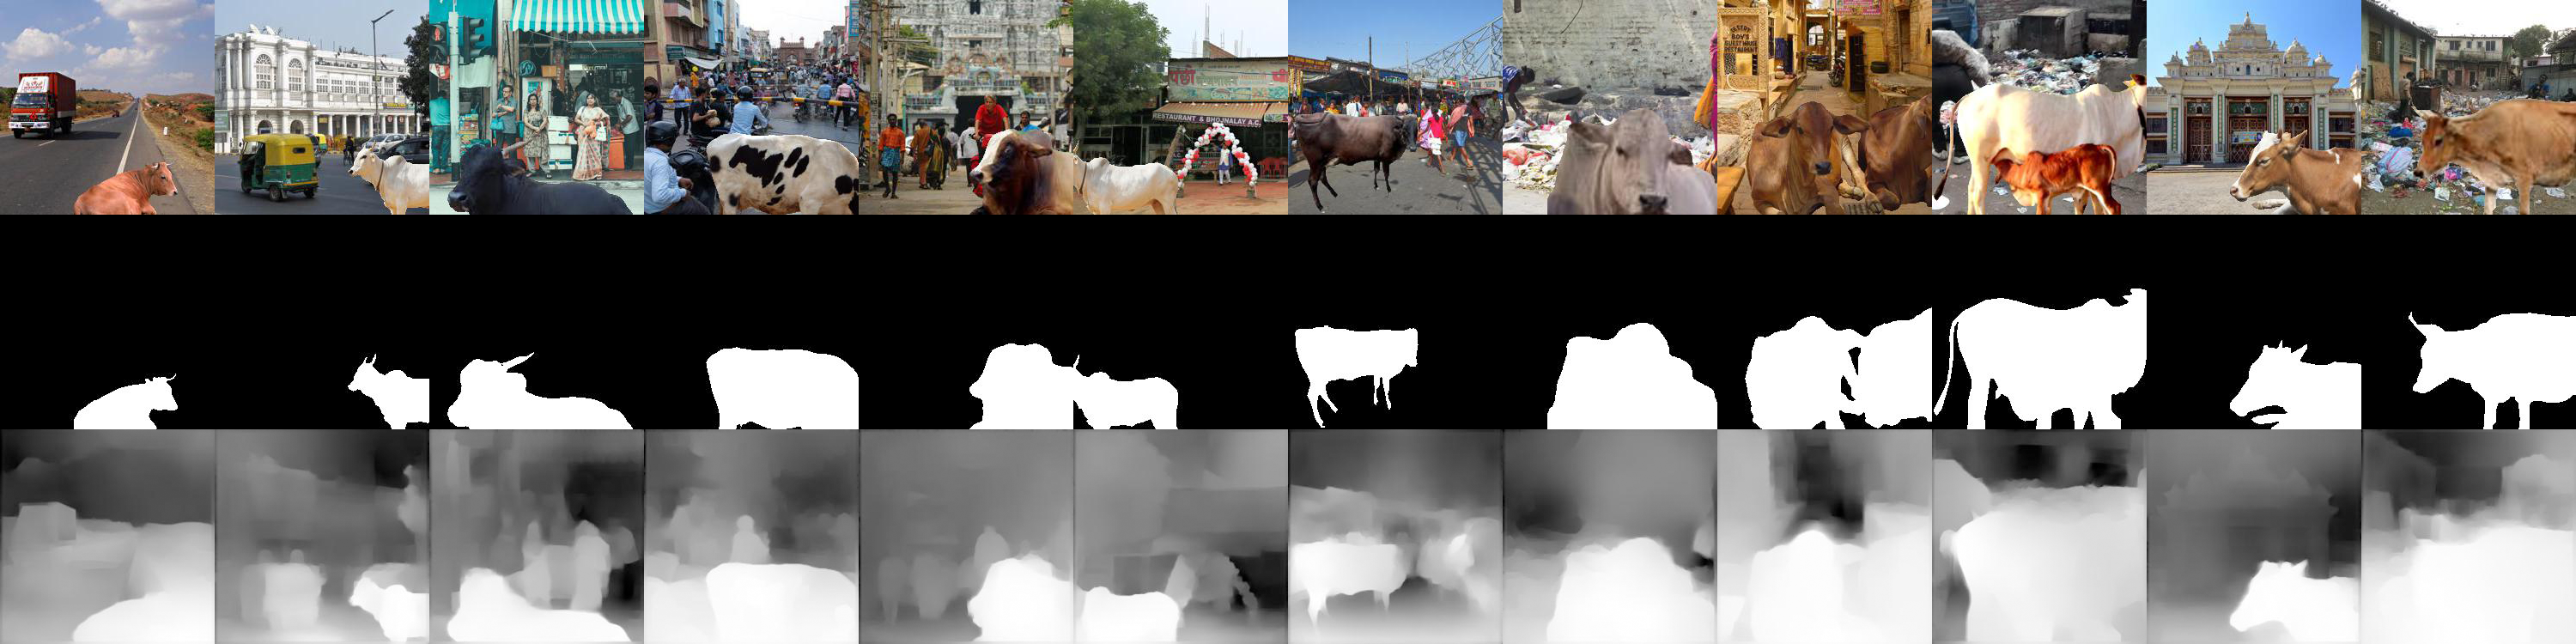
\includegraphics[width=1.0\linewidth]{good.png}
  \end{center}
  \caption{Three images resulted from the algorithm used. (top) A scene image on which a foreground object is positioned
   at random location with random scale, (middle) respective mask for the scene image, and (bottom) calculated depth by using a model.}
  \label{fig:finaldataset}
\end{figure*}

\section{Experiments}
In this section, we provide a baseline for monocular depth estimation and foreground segmentation on the \textit{SmallDepthMask} dataset.
Convolutional Neural Networks(CNN) are progressive in exploring structural features and spatial image formation. 
To come up with baseline, we started  training simple CNN, Resnet, and Unet++. 
The state-of-the-art models for image segmentation are variants of U-Net and fully convolutional networks (FCN)\cite{drozdzal2016importance}. 
long skip connections are used to skip features from the contracting path to the expanding path in order to recover 
spatial information lost during downsampling \cite{zhou2019unet++}. Short skip connections can be used to build deep FCNs. 

\subsection{Detecting Cattle on Road}

DISCUSS WHY? NEED FOR THIS APPLICaTION HERE...

Previous sections desribe as an example the dataset generation for this application. The dataset is available for public use. Every image (fgbg, mask, depth) in the dataset are of size $224\times224$. The distribution of fgbg, mask and depth values for XYZ dataset are shown in fig. (WHAT?). The dataset has $400K$ records. A $70-30$ train-test-split $280K$ and $120K$ train/test images respectively. 
A sample record in the dataset contains paths to all the images as shown below.

\textit{('./data/bgimages/bgimg099.jpg', 
'./data/out2/images/fgbg392483.jpg', 
'./data/out2/masks/mask392483.jpg', 
'./data/out2/depth/fgbg392483.jpg')}

\subsection{Model}
By using both long and short skip connections we proposed a light weight model following U-Net architecture with two decoder 
networks meant for segmentation mask prediction and depth prediction. The architecture of the model is shown in Fig \ref{fig:modelarch}. 
The total number of parameters of this model are $5,525,568$ including both the decoders. 

The encoder part of network is comprised of four DownSampling units. Every downsampling unit compresses the input scene image with the help of a series of convolutional operations. In our implementation, the source image of size $128 X 128$, changed into $64X64 \rightarrow 32X32 \rightarrow  16X16 \rightarrow 8X8$. This model has DepthDecoder and MaskDecoder and each of them is comprised of four upsampling units. The compressed source image is expanded with the help of Atrous and Transposed convolution operations. The encoder outcome $8 X 8$ is expanded into $16X16 \rightarrow 32X32 \rightarrow 64X64 \rightarrow 128X128$. As shown in model architecture Fig.\ref{fig:modelarch} the outcome of encoder downsampling units were added to outcomes of decoder upsampling units.

We have trained this model on the entire \textit{SmallDepthMask} dataset from scratch with train-test-split of $70-30\%$. 
During training the network is trained with the batch size of 64 for 10 epochs using SGD optimizer\cite{bottou2010large}. Every epoch took one hour of time on GPU because of the huge training data.
We have used OneCycleLR scheduler \cite{smith2018disciplined} with a maximum Learning rate of 0.1. 
This made the initial learning rate as 0.0099.
The Deep Convolutional Neural Networks encoder is fed with a image $(128 X 128)$ and the first decoder outputs a mask 
image and and second decoder outputs a depth image. To reduce overfitting\cite{perez2017effectiveness}, and achieve generalization
this work employed the augmentation techniques, Random Rotation, Random Grayscale, Color Jitter, random horizontal flips and random channel swaps. 

\begin{figure}
\centering
  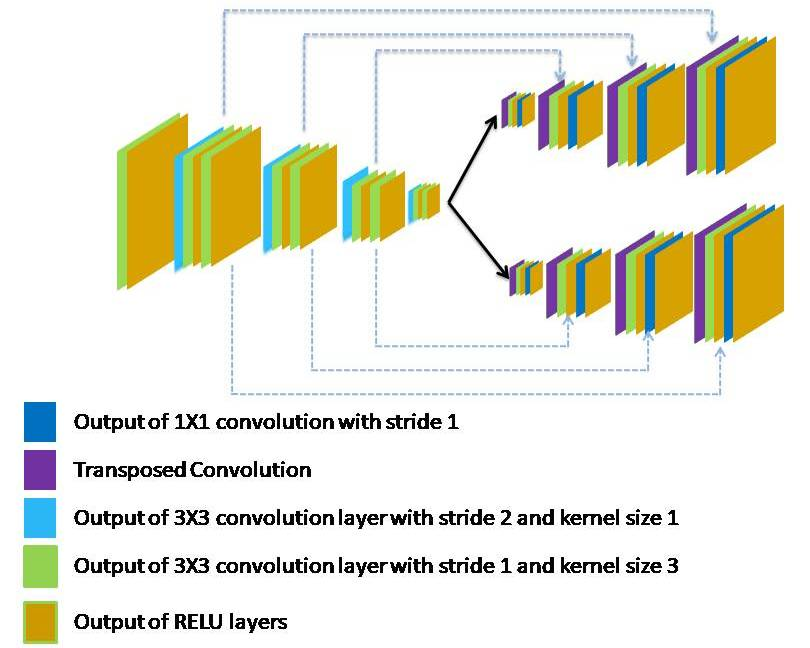
\includegraphics[width=1.0\linewidth]{networkarchitecture.jpg}
  \caption{Network Architecture}
  \label{fig:modelarch}
\end{figure}

\subsection{Loss function}
Deciding a universal loss function is not possible for complex objectives like Image segmentation and depth prediction. Based on the survey done by Shruti Jadon~\cite{jadon2020survey} we have picked L1 loss and SSIM(Structural Similarity Index) loss~\cite{zhao2015loss}. Their work also suggested to use penalty term which helps the network to focus towards hard-to-segment boundary regions. The Loss is calculated with the help of L1 and SSIM at both the decoders and employed regularization for weight penality.

For training our network with two decoders, we defined the same loss function $L$ for depth and mask prediction, between $y$ and $\hat{y}$ as the weighted sum of two loss function values.

\begin{equation}
L(y, \hat{y}) = \lambda L_{term1}(y, \hat{y}) + (1 - \lambda) L_{term2}(y, \hat{y})
\end{equation}

The first loss term $L_{term1}(y, \hat{y})$ is the point-wise L1 loss defined on the predictions of Mask Decoder and  
Depth Decoder units of the network.

\begin{equation}
L_{term1}(y, \hat{y}) = \frac{1}{n} \sum_{x=1}^{n} \mid y_i - \hat{y_i} \mid
\end{equation}

The second loss term $L_{term2}(y, \hat{y})$ uses a commonly used metric for image reconstruction task i.e., SSIM. 
Many recent toody depth prediction CNNs employed this metric. 
The loss term is redefined as shown in equation as SSIM has an upper bound of one.

\begin{equation}
L_{term1}(y, \hat{y}) = \frac{1 - SSIM(y, \hat{y})}{2}
\end{equation}

Different weight parameters $\lambda$ were tried and we have ended with a value $\lambda = 0.84$. The final loss function is as follows.

\begin{equation}
L(y, \hat{y}) = 0.84 \ast L_{term1}(y, \hat{y}) + 0.16 \ast L_{term2}(y, \hat{y})
\end{equation}

\subsection{Optimizer and Learning Rate}
MENTION DETAILS HERE

\subsection{Results}
The model is trained on the entire dataset and obtained significant accuracy and minimal loss. The outcome of the model on validation dataset is shown in Fig \ref{fig:validinfer}. and on the unseen data is shown in Fig \ref{fig:unseeninfer}. The unseen data fed to the model is a real picture and not one curated as in \textit{SamllDepthMask} where forgerround is placed on background. From the obtained segmentation masks and depths, It is very clear that the model generalized well. Few exceptions like the spots on cow and two calves not having very good detection indicate the non-presence of such examples in the training set. However, it should be straighforward to introduse few more examples to make the application more robust.

\begin{figure*}
  \begin{center}
    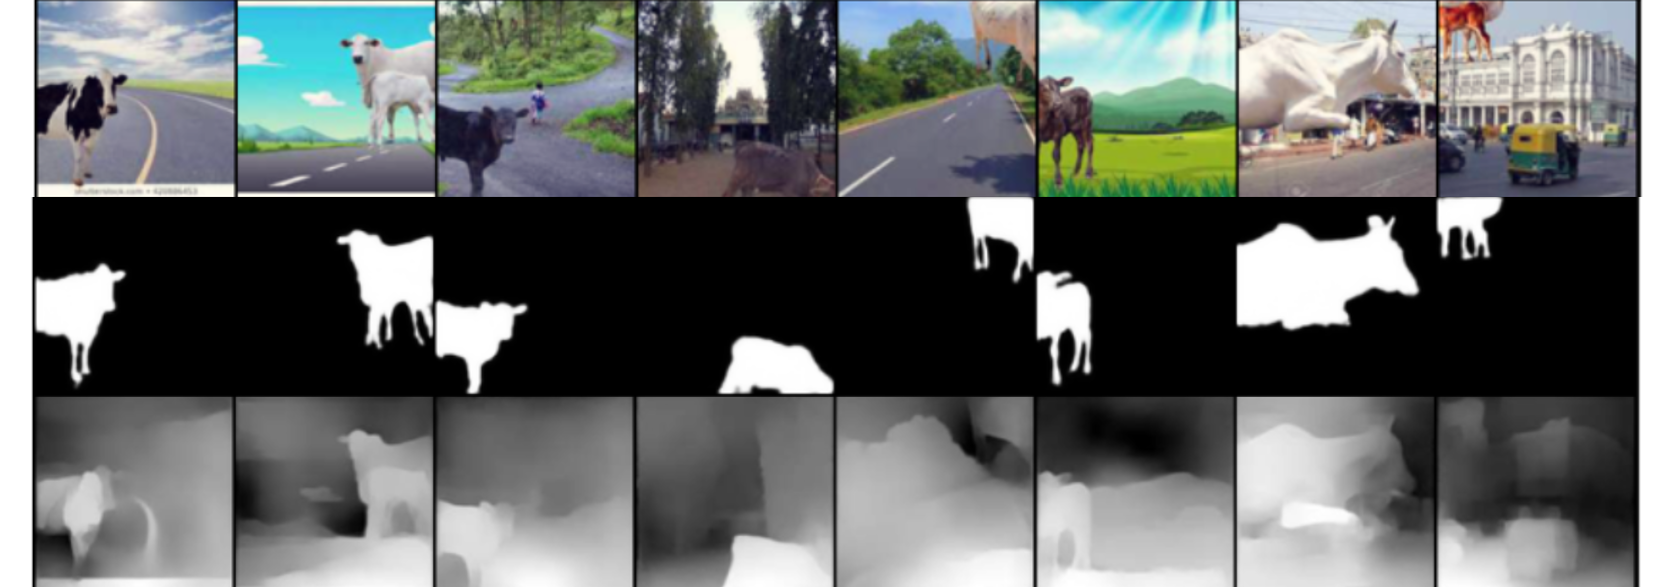
\includegraphics[width=1\textwidth]{validinference.png}
  \end{center}
  \caption{Segmentation mask and depth inference on validation data}
  \label{fig:validinfer}
\end{figure*}


\begin{figure*}
  \begin{center}
    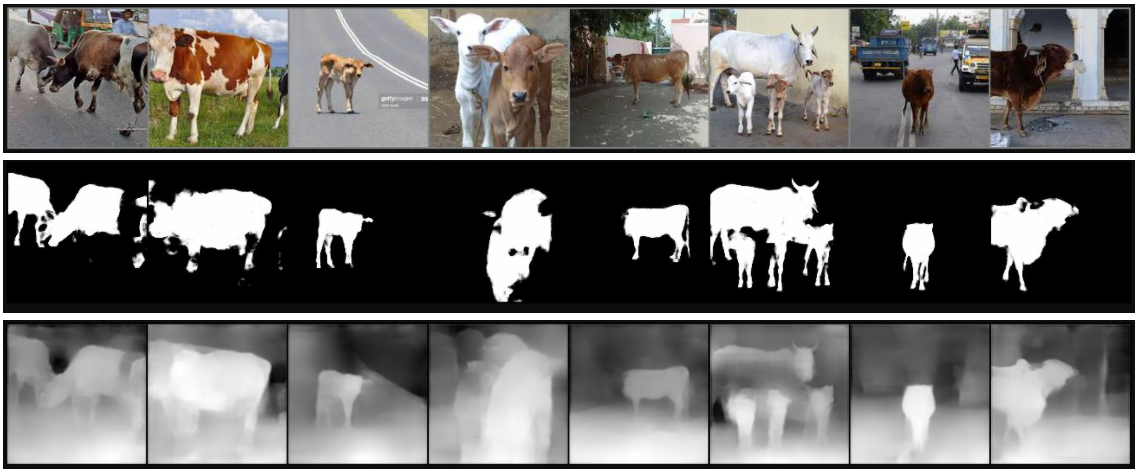
\includegraphics[width=1\textwidth]{unseeninference.png}
  \end{center}
  \caption{Segmentation mask and depth inference on unseen data.}
  \label{fig:unseeninfer}
\end{figure*}

\section{Conclusion and Future Work}
WRITE MORE HERE HOW WE FULFILLED THE CLAIMS
Robust dataset for Image Segmentation and depth generation is proposed whose implementation cost is low.
A lightweight baseline model to infer both mask and depth is proposed.

\begin{figure*}
  \begin{center}
  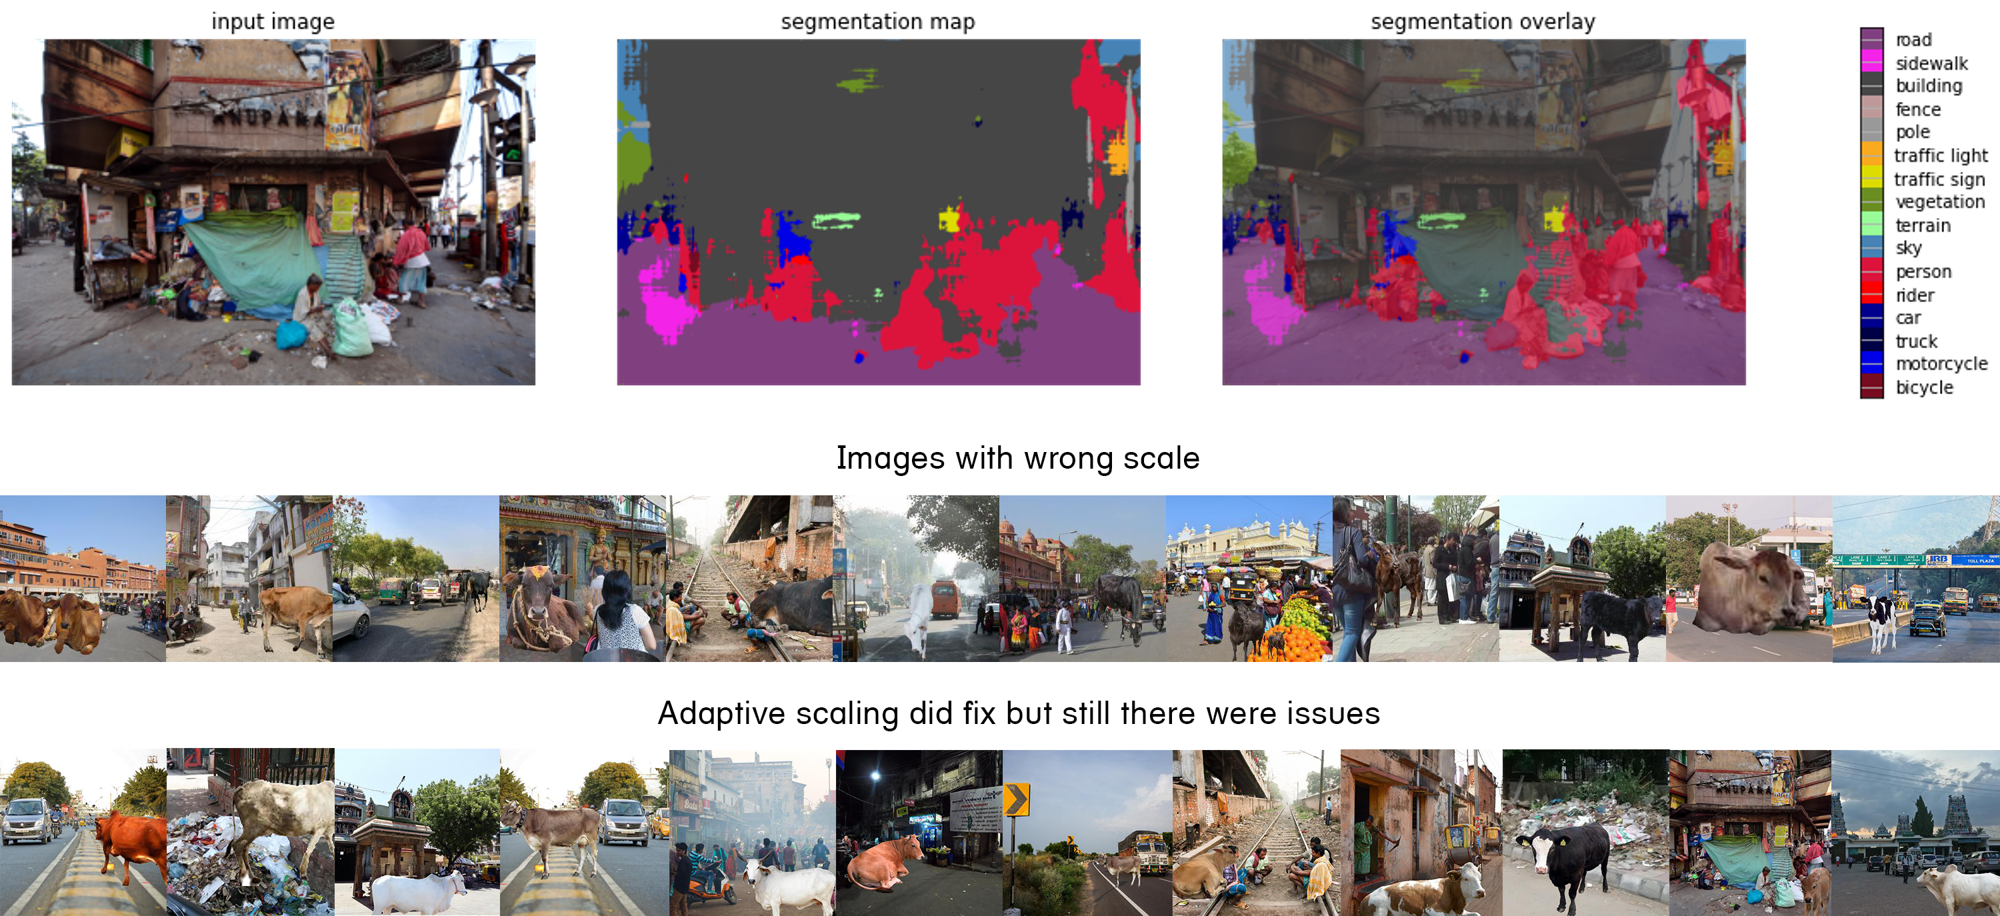
\includegraphics[width=1.0\textwidth]{refinement.png}
  \caption{Using Semantic Segmentation for adaptive placement and scaling. (Top) semantic segmentation. (Middle) Example of poor scaling and placement in proposed approach. (Bottom) Attempted correct placement and scaling}
  
  \end{center}
  \label{fig:refinement}
\end{figure*}

\begin{figure}
  \begin{center}
  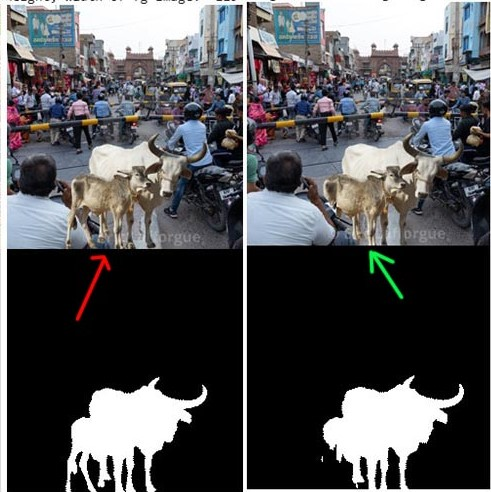
\includegraphics[width=1.0\linewidth]{occlusion.jpg}
  \caption{Restoring occlusion from semantic segmentation}
  \end{center}
  \label{fig:occlusion}
\end{figure}

Due to random scaling and placement the fg-bg images are often not so realistic. Figure \ref{fig:refinement} middle show sample images with wrong placement and scale. Regardless of this, the trained model is generalizing well. However, we experimented with detection of ground and sky regions from semantic segmentation. [ONE LINE WITH REFERECE TO THE WORK WE USED FOR THIS] That combined with the depth information of the background gives necessary cues as to where to place the foreground image and at what scale. Figure \ref{fig:refinement} shows the outcomes. We further experimented with adding occlusions from semantic segmentation information where non ground/sky pixels that belong to regions starting below the top margin of the foreground location, are placed on top of the foreground. Figure \ref{fig:occlusion} illustrates this. The effect of such data on training is yet to be explored. At the same time, the generated images by such informed scaling and placement are also not free from artifacts. The orientation and unknown size of foregroung object pose a challenge, leading to use of several experimental constants in the transformation process. We would like to formalize that and analyze its outcome on training as future work.

\section{Acknowledgement}
Authors are grateful to Vishnu Institute of Technology for providing necessary infrastructure, and to Rohan Sravan of The School of AI for initiating the idea and providing necessary support to carry out the research.

{\small
\bibliographystyle{ieee_fullname}
\bibliography{references}
}

\end{document}
